\documentclass[UTF8]{ctexart}
\usepackage{amsmath}
\usepackage{graphicx}
\usepackage{minted}
\usepackage{hyperref}
\usepackage{fontspec}
\usepackage{float}
\usepackage[normalem]{ulem}

\useunder{\uline}{\ul}{}
\hypersetup{hidelinks}
\graphicspath{ {images/} }
\setmonofont{Fantasque Sans Mono}
\setCJKmonofont{Microsoft YaHei}
\setminted{tabsize=2, fontsize=\footnotesize}

\title{基于Android平台的天气预报系统的设计与实现\footnote{完整代码请参见https://github.com/sylxjtu/Tenki}}
\date{\today}
\author{沈俞霖, 李南辰}

\begin{document}
  \maketitle
  \vspace{80mm}
  \begin{flushright}

  \textbf{课程} \makebox[7em][l]{Android Java开发}

  \textbf{姓名} \makebox[7em][l]{沈俞霖}

                \makebox[7em][l]{李南辰}

  \textbf{学号} \makebox[7em][l]{2151601013}

                \makebox[7em][l]{2151601010}

  \textbf{日期} \makebox[7em][l]{\today}

  \end{flushright}
  \newpage

  \tableofcontents
  \newpage

  \section{问题定义}
    用户需要一款简单实用的天气应用,进行实况天气和天气预报的查看
  \section{需求分析}
    \begin{itemize}
      \item 要求应用可以获取用户的地理位置,精确到区级行政区,以便获取天气信息
      \item 要求应用给出用户所处地理位置的实时天气信息,即实时气温以及天气情况
      \item 要求应用给出用户所在地未来数天的早晚天气预报,所包含的信息应有:气温与天气
      \item 当应用正在获取天气信息需要用户等待时,应有相应提示
      \item 当应用无法获取天气信息时,应给出相应提示,并指出原因
    \end{itemize}
  \section{结构设计}
    \begin{itemize}
      \item 使用android自带api实现地理定位
      \item 使用网络上的api实现实况天气和天气预报
      \item 使用网络上的天气图标集实现天气图标显示
    \end{itemize}
  \section{编码实现}
    \subsection{JsonApiTask 实现从JSON的API接口获取数据的功能}
      \inputminted{java}{../app/src/main/java/com/sylxjtu/prototype/JsonApiTask.java}
    \subsection{MainActivity 实现程序主界面和定位功能}
      \inputminted{java}{../app/src/main/java/com/sylxjtu/prototype/MainActivity.java}
      \inputminted{xml}{../app/src/main/res/layout/activity_main.xml}
  \section{运行测试}
    \subsection{测试用例}
      \begin{itemize}
        \item 正常情况
        \item 不开启定位
        \item 不开启网络
      \end{itemize}
    \subsection{测试结果}
      \subsubsection{正常情况运行界面}
        \begin{figure}[H]
          \caption{正常情况运行界面}
          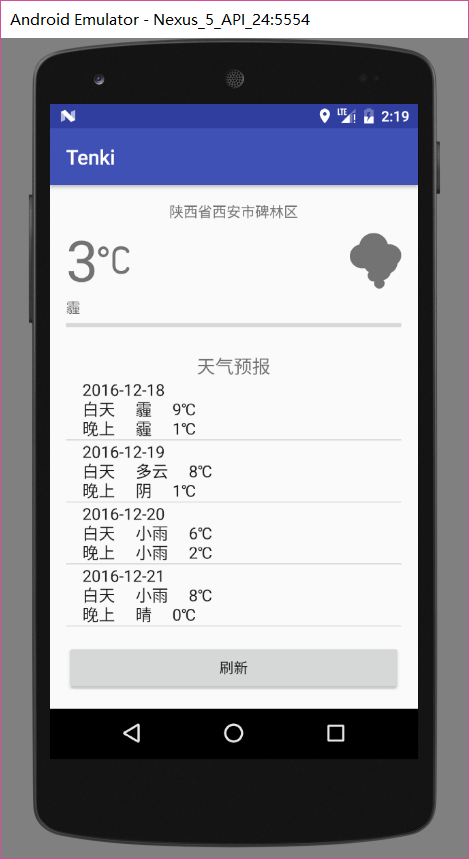
\includegraphics[width=\textwidth, height=40em, keepaspectratio]{正常情况运行界面}
          \centering
        \end{figure}
      \subsubsection{不开启定位情况下运行界面}
        \begin{figure}[H]
          \caption{不开启定位情况下运行界面}
          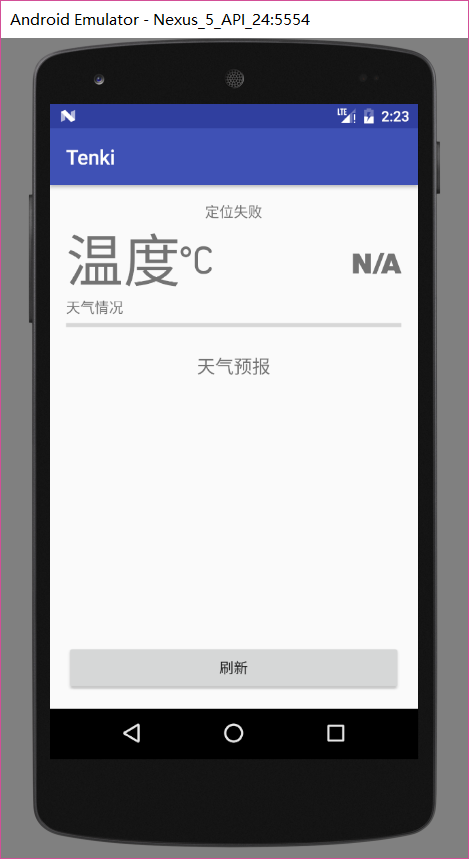
\includegraphics[width=\textwidth, height=40em, keepaspectratio]{不开启定位情况下运行界面}
          \centering
        \end{figure}
      \subsubsection{不开启网络情况下运行界面}
        \begin{figure}[H]
          \caption{不开启网络情况下运行界面}
          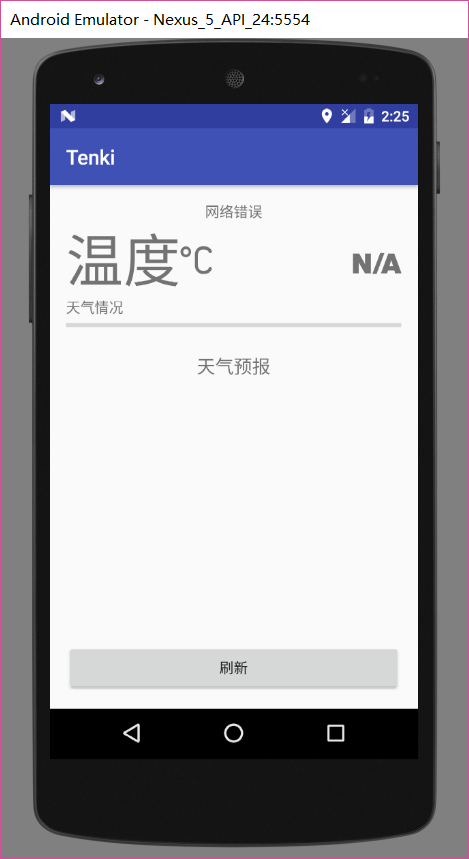
\includegraphics[width=\textwidth, height=40em, keepaspectratio]{不开启网络情况下运行界面}
          \centering
        \end{figure}
\end{document}
